\chapter{Thesis Advancement}
\label{chap:context}
\minitoc

\section{Context and motivation}
%
Combining data from different data sources (known in advance) and providing 
a unified view of the result to data consumers is a well-known problem in 
database theory called data integration. 
%
Many authors have proposed algorithms for rewriting a data consumer query
according to different views expressed over different database schemas.
%
In general, these approaches are expensive in terms of computing resources
sharing the 
same performance problem while combining the different query concepts 
in order to produce a rewrite according to the expectations. 

Data integration solutions could take advantages from cloud architectures.
%
Cloud providers deliver on-demand computing resources to cloud consumers
(for example, an end-user, a data service or another cloud)
according to the quality of service they have agreed in a service level 
agreement (SLA) contract. 
%
An SLA states what the data consumer can expect from a service or a system
behavior.

Data integration can be seen in the cloud computing as a service matching 
and composition problem which implies consuming data from different data 
services and integrating results. 
%
Researches in this domain also deal with problema de processamento ...have proposed 

\bigskip
Data services and data processing services can be deployed in cloud infrastructures under different quality measures. Such measures describe the conditions in which a service can provide or process data. These measures can be expressed in a service level agreement (SLA), which states what the user can expect from a service or system behavior.
However, the current SLAs are mainly interested in performance aspects (such response time, availability, memory and others) putting aside data quality requirements (such as freshness, veracity, type and others).

%Data integration problem is widely studied in the database domain~\cite{Lenzerini:2002}. 
%Current data integration implies consuming data from different data services and integrating the results while meeting users' quality requirements. Such requirements include the data that is retrieved and integrated, but also the properties of the data, its producers and the conditions in which such data is produced and processed. For example, whether the user accepts to pay for data, its provenance, veracity and freshness and how much is the user ready to pay for the resources necessary for integrating her expected result. 

%Data services and data processing services can be deployed in cloud infrastructures under different quality measures. Such measures describe the conditions in which a service can provide or process data. These measures can be expressed in a service level agreement (SLA), which states what the user can expect from a service or system behavior.
%For example, whether it implements an authentication process, if it respects data consumer's privacy and the quality of the data the service can deliver, like freshness, veracity, reputation and other non-functional conditions like the business model that controls data delivery. 
%However, the current SLAs are mainly interested in performance aspects (such response time, availability, memory and others) putting aside data quality requirements (such as freshness, veracity, type and others).

%Data integration can be seen in the cloud computing as a service composition problem. 
%In our previous work~\cite{Carvalho2015}, we have identified that QoS aspects has started to be considered while integrating data, and the cloud has become a popular environment to perform data integration. Moreover, data integration combined with SLA is an open issue in the cloud. 
In this sense, the objective of this work is to address data integration in a multi-cloud context. 
The originality of our approach consists in guiding the entire data integration solution taking into consideration
(i) user preferences statements (regarding data quality requirements); 
(ii) infrastructure properties (reliability, computing, storage and memory capacity, and cost) imposed by the multi-cloud context; 
(iii) SLA contracts exported by different cloud providers; and 
(iv) several QoS measures associated to data collections properties (for instance, trust, privacy, economic cost).

%Thus, the \textbf{first challenge} is to compute what we call an integrated SLA that matches the user's integration preferences (including quality constraints and data requirements) with the SLA's provided by cloud services, given a specific user cloud subscription. The user may have general preferences depending on the context she wants to integrate her data such as economic cost, bandwidth limit, free services, and storage and processing limits. The SLA's associated to the cloud services can be of different types: user - data service, data service - cloud provider, data provision service - data processing service, and cloud provider - cloud provider. In this context, matching the user integration preferences with the services that can contribute to produce a result can lead to search and identify in the chain of SLAs. Probably it is possible to find an incompatibility between the preferences and a SLA in the chain, in this case it is necessary to propose a strategy to solve the problem. 
%
%Furthermore, in order to fulfill requirements and satisfy user expectations, it is possible to have a collaboration between different clouds. This collaboration implies the agreement through SLAs between services deployed in different cloud providers. In consequence, matching user preferences with SLA's can lead to deal with heterogeneous SLA specifications (different schemata, different measures semantics and granularities). Computing an integrated SLA can imply dealing with heterogeneous SLA specifications and SLA-preferences incompatibilities.

%The \textbf{second challenge} is to guide data integration taking into consideration the integrated SLA. Here, the data integration process includes (i) looking up services that can be used as data providers, and for services required to process retrieved data and build an integrated result; (ii) performing data retrieval, processing and integration and (iii) deliver results to the user considering her preferences (quality requirements, context and resources consumption). The integrated SLA can guide services filtering in the look up phase; it can help to control the amounts of data to retrieve and process according to consumption rights depending on the user subscription to the participating cloud providers and how to deliver data considering the user's context.

\section{Problem statement}
%
The multi-cloud architecture brings new challenges to data integration
and data processing applications.
%
Instead of taking into consideration the user query and his/her requirements
with respect to services' performance capabilities (such as percentage of 
availability and response time) in isolation, the integration process 
must consider in addition the new constraints imposed by context: 
%
\begin{itemize}
\renewcommand{\labelitemi}{$-$}
\item User requirements concerns not only data services' performance 
capabilities but also quality requirements of the data which is provided
(such as freshness, cost, provenance, data type, veracity among others).
%
\item Data provision is constrained to the available computing resources agreed
between data services and cloud providers on service level agreement (SLA) contracts. 
%
\item The data integration process requires a high level of computing resources.
The huge amount of data and data services on multi-cloud settings increases even 
more the complexity of the solutions.
\end{itemize}
%
In this sense, current data integration solutions introduces a multi-dimensional 
matching problem that should take into account:
%
\begin{itemize}
\renewcommand{\labelitemi}{$-$}
\item Expressing data consumer requirements with respect to performance 
capabilities of data services and to the quality of the expected data.
%
\item Matching and selecting data services according to the data consumer expectations 
(concerning performance and data quality requirements) with respect to data 
services quality measures defined in SLA contracts. 
%
\item Matching and selecting data services which have available resources according
to different SLAs that they have agreed with different cloud providers.
%
\item Delivering results with respect to the data consumer requirements and expectations 
depending on the context which he/she consumes the data.
\end{itemize}
%
Thus, the intention of this thesis project is to address data integration on multi-cloud 
environments.
%
The aim is propose a data integration approach adapted to the multi-cloud context in 
which data is delivered according to data consumers expectations by profiting from 
previous integration results instead of launching the expensive data integration 
process from the first step. 


\section{State of the Art}

The state of the art comprehend four topics: 
(i) data integration and data quality in the database domain; 
(ii) data integration approaches in the cloud and in service-oriented contexts; 
(iii) query rewriting approaches; and 
(iv) service level agreements for cloud computing.

Data integration has been widely discussed in the database domain.
It consists in merging data from different databases and providing a unified view of this data to the user.
\cite{Lenzerini:2002} discussed theoretical aspects in data integration including modeling applications, query evaluation, dealing with inconsistencies and reasoning queries.
Moreover, \cite{Halevy:2001} reviewed several query rewriting approaches. 
\cite{Batini2006} surveyed data quality aspects in data integration systems. 
\cite{Scannapieco:2004} presented a data quality broker that allows to submit queries with associated quality requirements over a global schema and to provide results according to them.

\cite{Correndo2010,ElSheikh2013} performed data integration in service-oriented contexts, particularly considering data services. However, they  consider computing resources consumption versus performance for guiding the data integration process. 
%\cite{YauY08} addressed data privacy  to integrate data collected from different data services. 
\cite{Tian2010} proposed an inter-cloud data integration system considering privacy requirements and the cost for protecting and processing data. 
\cite{Scannapieco:2004,Tian2010,YauY08} tackled quality aspects of the integration, but do not consider crucial aspects such as data consumers and data providers requirements and constraints, the associated infrastructures and the data quality itself. %It is also important to include these criteria in the way services are composed to produce  query plans.

As traditional databases theory, data integration on cloud and service-oriented context deals with query rewriting issues. Existing works like~\cite{ba2014,Barhamgi2010,Benouaret2011,Umberto} have refered it as a service composition problem. Given a query, the objective is to lookup and compose data services that can contribute to produce a result. In general, these works must address performance issues, because they use algorithms that can become expensive according to the complexity of the query and on the number of available services. Although \cite{ba2014,Benouaret2011} have considered preferences and scores to produce rewritings, the multi-cloud context introduces new requirements and constraints to the integration process. Currently, the approaches are not sufficient to cover the new challenges. Thus, they should be revisited and adapted in order to make the integration efficient in this new environment. 

Several researches have reported their studies on SLA in different domains~\cite{AlhamadDC11}.
Contributions related to SLA in cloud computing concern (i) SLA management~\cite{Mavrogeorgi2013}; 
(ii) inclusion of security requirements on SLAs~\cite{rak2013}; (iii) SLA negotiation~\cite{Falasi2016, Son2014}; (iv) SLA matching~\cite{Redl2012}; and (v) monitoring and allocation of cloud resources to detect and avoid SLA violations~\cite{Leitner2010}. 
These contributions are mainly focusing on performance aspects (for example, response time, memory, VMs allocation and others) in their SLA rather than quality issues regarding the delivered data itself (for example, data type, freshness, provenance and others).
Thus, we strongly believe that SLAs can be used  to explicitly introduce the notion of quality in the current data integration solutions. 
In this sense, the use of SLAs to guide the entire data integration in a multi-cloud context seems original and promising for providing new perspectives to the data integration problem.

% In the cloud context, Rak \textit{et al.} proposed an approach to specify security requirement and to associate them to cloud services~\cite{rak2013}. Mavrogeorgi \textit{et al.} introduced a SLA management framework that allows the creation and enforcement of customized SLAs~\cite{Mavrogeorgi2013}. Leitner \textit{et al.} presented an approach to monitor and predict SLA violations before they impacted the provider's SLA~\cite{Leitner2010}. In general, proposals regarding SLAs in the deployment of services focus on two aspects: (\textit{i}) approaches focusing on the life cycle of the SLA mainly interested in the contract negotiation phase between the cloud and the service consumer; and (\textit{ii}) works monitoring contracts and cloud resources in order to avoid SLA violations, and consequently penalties due to its violation. In this sense, to the best of our knowledge, we have not identified any other approach that proposes the use of SLA associated to a data integration solution in a multi-cloud environment.



\section{Synthesis of the work}
%
%
\subsection{First year}

During the first year of project, we have been working on the state of the art. The idea is to be aware of all types of publications close related to the thesis proposal. To reach this, we proceeded with a literature analysis using a systematic mapping methodology. 
	
Briefly, the methodology consists in retrieving papers from scientific databases using the same search string. 
These papers are filtered according to an inclusion and exclusion criteria that should be defined based on the research interests. 
The papers will be classified in different categories (called facets) and for each facet in a specific dimension. 
The facets and dimension are defined based on the authors' knowledge and interests. 
Taking the final papers collection, the abstracts should be read in order to classify each paper into the dimensions for each facet. 
This methodology allowed us to identify trends and open issues regarding our research topic and proposing an approach that fills some gaps and proposes an original data integration solution according to current trends in the area.
The table~\ref{table:sysmap} presents our results. We retrieved 1832 papers. 114 papers were selected based on our inclusion and exclusion criteria.
As result of this work, we have published a paper on DEXA 2015 (See annex~\ref{chap:appendix1}).

\begin{table}
\center
\begin{tabular}{|c|c|c|c|}
\hline 
\textbf{Database} & \textbf{Amount} & \textbf{Include} & \textbf{Excluded} \\ 
\hline 
\textit{IEEE} & 658 & 56 & 602 \\ 
\hline 
\textit{ACM} & 649 & 31 & 618 \\ 
\hline 
\textit{Science Direct} & 106 & 6 & 100 \\ 
\hline 
\textit{CiteSeerX} & 419 & 21 & 398 \\ 
\hline 
\textit{Total} & 1832 & \underline{114} & 1718 \\ 
\hline 
\end{tabular} 
\caption{Systematic Mapping: sumary of paper per databse.}\label{table:sysmap}
\end{table} 

\subsection{Second year}

During the second year, we have been working on the development of our data integration approach. Given a query and a set of user preferences associated to it, the query execution process is divided in three phases. The figure 1 illustrates our data integration approach.

\begin{figure}[h!]
\center
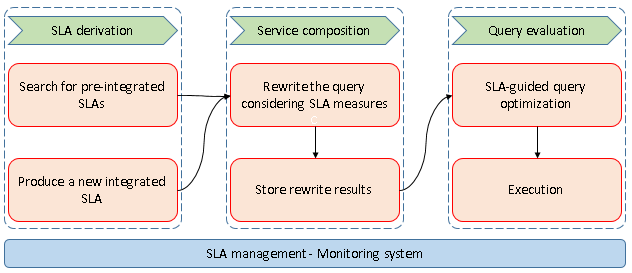
\includegraphics[scale=0.7]{/images/general_approach.PNG} 
\caption{SLA-guided data integration approach}
\end{figure}

\underline{The first phase} is the SLA derivation in which a SLA for the user request is created. It consists in looking for a (stored, integrated) SLA derived for a similar request. If a similar SLA is found, the request is forwarded to the query evaluation phase. Otherwise, a new SLA to the integration (called integrated SLA) is produced. The query is expressed as a service composition with associated user preferences. In \underline{the second phase}, service composition, the query is rewritten in terms of different services considering the user preferences and the SLAs of each service involved in the composition. The rewriting result is stored for further uses. \underline{Finally}, in the query evaluation phase, the query is optimized in terms of user preferences and SLAs concerning the consumed resources and the economic cost of the query. Once optimized, the query processed in the execution engine. In addition, we are assuming a SLA management module and monitoring system responsible to verify if the SLA contracts are being respected. Firstly, we have worked on the phases two in order to have an algorithm that will allow us to run important experiments to evaluate our approach. 
%The following activities were developed to achieve our objectives:
	
\cite{ba2014} have proposed an algorithm for refining services composition. Their goal was to use user preferences to select and rank services in order to avoid the exponential problem while combining and producing compositions. Composition are incrementally produced until to reach a (predefined) desired number. In collaboration with our colleagues in Brazil (authors in~\cite{ba2014}), we have worked on an adapted version of \cite{ba2014} to our data integration solution extending their data structure to map services to the query, and adding the concepts of user preferences to the query and quality measures to the services. However, while performing the integration we have identified some design issues that made it useless to our approach: (i) their concept of user preferences are scores associated to services previous defined by the user while, for us, user preferences are quality requirements expected by the user concerning the whole integration; (ii) their algorithm accepts rewriting including calls to services that are not interest for the composition. Assuming that on the cloud each service has a price associated to its request, these composition that calls useless services produces an extra cost to the user. This adaptation process helped us to identify important issues to be applied to our own implementation such as developing an better approach to produce the combinations of services.

%a) Adapting a previous query rewriting algorithm to our approach. This work was performed in collaboration with our colleagues in Brazil. The idea was to adapt a previous work from their lab to our data integration solution. While integrating we have identified some design problems that made it useless to our approach. However, the work in group help us to identify important issues to be applied to our own implementation.

%b) Query rewriting algorithms. We have produced a state of the art about query rewriting algorithm.  The approaches are divided into two different domains: database and service-oriented architecture. In the database domain, the different works concerning query rewriting using views have been studied in the literature. In general, the approaches deal with an exponential problem depending on the size of the query and the quantity of views. In the service-oriented domain, the approaches share the same problem. Producing services composition is extremely costly depending on the size of the composition (query) and the amount of services to be combined. Some approaches have tackled this issue. They have tried to minimize the effort to produce rewritings by considering user preferences or by limiting the desired number of rewritings. These works have been used as base and reference to produce our own algorithm.

%Starting from the knowledge acquired while working on~\cite{ba2014}, we have produced a state of the art about query rewriting algorithm. The approaches can be divided into two domains: database and service-oriented architecture. In the database domain, studies (such as \cite{Duschka:1997,Levy:1996,Pottinger:2001}) have documented their approaches for answering queries using views. In general, while producing rewritings, these approaches suffer from the time exponential problem depending on the size of the query and the quantity of views. In the service-oriented domain, query rewriting can be seen as a service composition problem. Approaches (such as \cite{Barhamgi2010,Benouaret2011,Umberto}) share the same problem as on the database domain while producing services composition which is a task extremely costly depending on the size of the composition (query) and the amount of services to be combined. \cite{ba2014} have tried to minimize the effort to produce rewritings by considering user preferences (as scores) and by limiting the desired number of rewritings.

%Based on the related work, we have developed and formalized the \textit{Rhone} service-based query rewriting algorithm guided by service level agreements (SLA).
Based on the related work, we have developed and formalized the \textit{Rhone} service-based query rewriting algorithm guided by service level agreements (SLA). The \textit{Rhone} assumes that there are a set of quality measures associated to services which we suppose they are previously extract from their SLA. These measures will guide the service selection and the entire rewriting process.  Our work address this issue and proposes the algorithm with two original aspects: (i) the user can express her quality preferences and associated them to his query; and (ii) service's quality aspects defined in SLAs guide the service selection and the whole rewriting process taking into consideration that services and rewritings should meet the user requirements, and the different cases of incompatibilities of SLAs, uncompleted SLA and the integration SLA. 
%and (ii) while trying to fulfill the user quality preferences, service’s quality aspects defined in SLAs guide the service selection and the whole rewriting process (Services and rewritings should meet the user requirements).
Given a set of abstract services, a set of concrete services and a user query (both defined in terms of abstract services), and a set of user quality preferences, the \textit{Rhone} derives a set of service compositions that answer the query and that fulfill the quality preferences regarding the context of data service deployment. The algorithm consists in four steps: (i) \textit{Selecting concrete services}. Similar to~\cite{Levy:1996,Pottinger:2001} our algorithm selects services based on the abstract services that exists in the query, but it includes two differences: first, a concrete service cannot be select if it contains an abstract service that is not present in the query; and second, the service' quality aspects (extracted from its SLA) must be in accordance with the user quality preferences; (ii) \textit{creating mappings from concrete services to the query (called concrete service description (CSD))} inspired in~\cite{Pottinger:2001} including also the information concerning the services' SLA; (iii) \textit{combining CSDs}; and (iv) \textit{producing rewritings} until fulfilling the user requirements according to the services' SLA. Each phase of the algorithm and each concept (query, concrete services, mapping rules, for instance) were formally specified and described. As result to this work, we have published a paper on ADBIS 2016 (See annex~\ref{chap:appendix2}).

%d) Configuration of a multi-cloud environment. We have worked on the configuration of a multi-cloud environment. However, we found some problems at this point: (i) the configuration and deployment of cloud infrastructure using open source technologies is not easy and requires important technical skills while configuring the network resources; (ii) it requires a powerful machine. Due to that we have configured a simulation of cloud; and (iii) we have searched for private cloud providers, but they allow few access and power permissions to manage resources. In addition, they are quite expensive. We are still working on best way to manage this issue.
\bigskip
In order to evaluate our approach and the \textit{Rhone} algorithm, we began configuring a multi-cloud environment. We have searched for open source solutions instead of privates once they are (i) quite expensive; and (ii) do not allow to extend and access directly the different level of SLAs. The OpenStack was selected as our technology. We have installed and configured the different modules necessaries to the OpenStack. However, we have some issues: (i) the configuration and deployment of cloud infrastructure require important technical skills while configuring the network resources; (ii) it requires a powerful machine. Due to these reasons we have configured a simulation of cloud run our experiments.

\textit{Rhone} was implemented using Java according to its formal definition. The algorithm was tested in a cloud simulation containing 100 services in its service registry. We have tested different types of query varying on the size and on the number of user preferences. Although our algorithm shares the same time performance problem as the previous approaches while combining compositions, the experiments have shown that the \textit{Rhone} can enhance the quality and reduce the cost in data integration by considering the user preferences and service's quality aspects extracted from service level agreements.
The results can be found in the annex~\ref{chap:appendix2}.
 

%We developed an improved version of the algorithm that better manages the manner in which lists of objects are managed. We have applied this version to a new set of experiments running 100 concrete services. With the results obtained from this experiment and the final version of our formalization, we are working on a new paper that included an extensive description of the algorithm and its evaluation to be submitted to ADBIS 2016 (deadline 27th March).

%h) SLA model to data integration. The state of the art on SLA have been analyzed to serve as basis to our SLA model. The works on SLA to cloud computing can be divided in two groups: (i) approaches dealing with the SLA negotiation phase. They focus on methods to stablish good and well-defined agreements between providers and customers; and (ii) works focus on monitoring/allocating resources in order to detect and avoid SLA violations. These works helped while proposing our SLA model and schema. Note that the SLA is the main concept in our proposal. It is responsible to guide the entire approach from the beginning to the end. There are some challenges regarding SLA: (i) once we are inserted into a multi-cloud context, we are dealing with a large heterogeneity of SLAs among different clouds. It is possible to have the same concept defined in a different way depending on the cloud; (ii) there are different levels of SLA: user SLAs, service SLAs and cloud SLAs. It is necessary to have a mapping between SLA measures that can be expressed in a different manner depending on the level; and (iii) it is possible to face a diversity chain of SLA from different levels and to map and identify measures is a hard process.

Moreover, we have designed \textit{(i)} a meta-model to data integration on multi-cloud environment and \textit{(ii)} schemas for user' SLA and cloud' SLA.
The meta-model has improved the scenario description to illustrate our approach.
As result of this work, we had a paper accept in the ICSOC PhD Symposium 2016 (See annex~\ref{chap:appendix3}).

%With this work performed, we have been designing our SLA model to data integration. As mentioned before, proposals to SLA in cloud computing can be divided in two groups: (i) approaches dealing with the SLA negotiation phase. They focus on methods to establish good and well-defined agreements between providers and customers; and (ii) works focus on monitoring/allocating resources in order to detect and avoid SLA violations. These works helped us while proposing our SLA model and schema. The SLA is the main concept in our proposal. It is responsible to guide the entire approach from the beginning to the end while fulfilling the user requirements. At this point, some challenges arises: (i) In a multi-cloud context, we are dealing with a large heterogeneity of SLAs among different clouds in terms of semantics and structure. A SLA and its measure can be defined in a different way depending on the cloud; (ii) there are different levels of SLA: between users and services, between services and clouds, between clouds and clouds. Consequently, a user requirement defined in a user SLA is computed in terms of different measures on Service and Cloud SLAs. It is necessary to have a mechanism that maps and compute the user requirement and SLA measures; and (iii) it is possible to exists a chain of SLA, and to map and computed measures in this chain can require a hard processing. i) Paper to ADBIS and VLDB PhD consortium. Currently, we have been working on a paper that focus on the description of our SLA model, schema and data integration approach to be submitted to the VLDB PhD workshop (deadline 4 April).

%i) Paper to ADBIS and VLDB PhD consortium. Currently, with our last results, we have been working on two new papers: one concerning the algorithm to be submitted to ADBIS 2016 (deadline 27th March), and another one focusing on the SLA model, schema and data integration approach to be submitted to the VLDB PhD workshop (deadline 4 April).

\subsection{Third year}

In the third year, we have worked on the following activities: 
\begin{enumerate} [a)]
\item Identifying related works on heuristics to service selection. As result, proposing a heuristic to \textit{(i)} service selection and ranking, but also to \textit{(ii)} rank compositions based on the services' SLA measures.
\item Definition and formalization of a taxonomy of queries treated by the integration approach.
\item Definition and formalization of reusability aspects applied to the query taxonomy in order to profit from previous integration results. 
\item Design of a data model to our query history.
\item Implementation of the query history and adaptation of the \textit{Rhone} algorithm to process its queries based on the data model.
\end{enumerate}

Ongoing work: 
\begin{enumerate} [a)]
\item Extending the \textit{Rhone} to include the reusability functions and run new experiments, and compare them to the previous results.
\item Improving the formalization aspects and performing corrections.
\end{enumerate}

As result to this work, we are planning to write a paper to the 36th International Conference on Conceptual Modeling (ER 2017) -- to be submitted in 17th April.